% !TeX root = ../thuthesis-example.tex

\chapter{绪论}

本章节分析了现有的固定路线定位技术的研究背景和研究意义,介绍了国内外关于视觉惯性定位和地图辅助定位的研究现状,并指出了现有研究的不足之处。本章通过论述核心研究内容,提炼出了文章的创新之处;简要介绍了整个系统的总体设计与其对应的研究内容;最后,给出了本文的组织结构。


\section{课题背景}

近年来,汽车和机器人的智能化是炙手可热的研究领域,而固定路线下运行的智能汽车和机器人是其中的一个重要研究和应用方向。相较于通用智能,在固定路线下应用的智能化技术更容易实现,因此固定路线场景下的应用涌现,例如图~\ref{fig:apply} 中所示的无人驾驶公交车\cite{stephen2023driverless}、智驾汽车通勤模式\cite{xin2023xinchuxing}、变电站巡检车\cite{song2020xinhuawang}、矿山无人运输机器人\cite{li2023keji}等,都是目前固定路线智能体的典型应用场景。

\begin{figure}[htbp]
  \centering
  \begin{subfigure}[b]{0.45\textwidth}
      \centering
      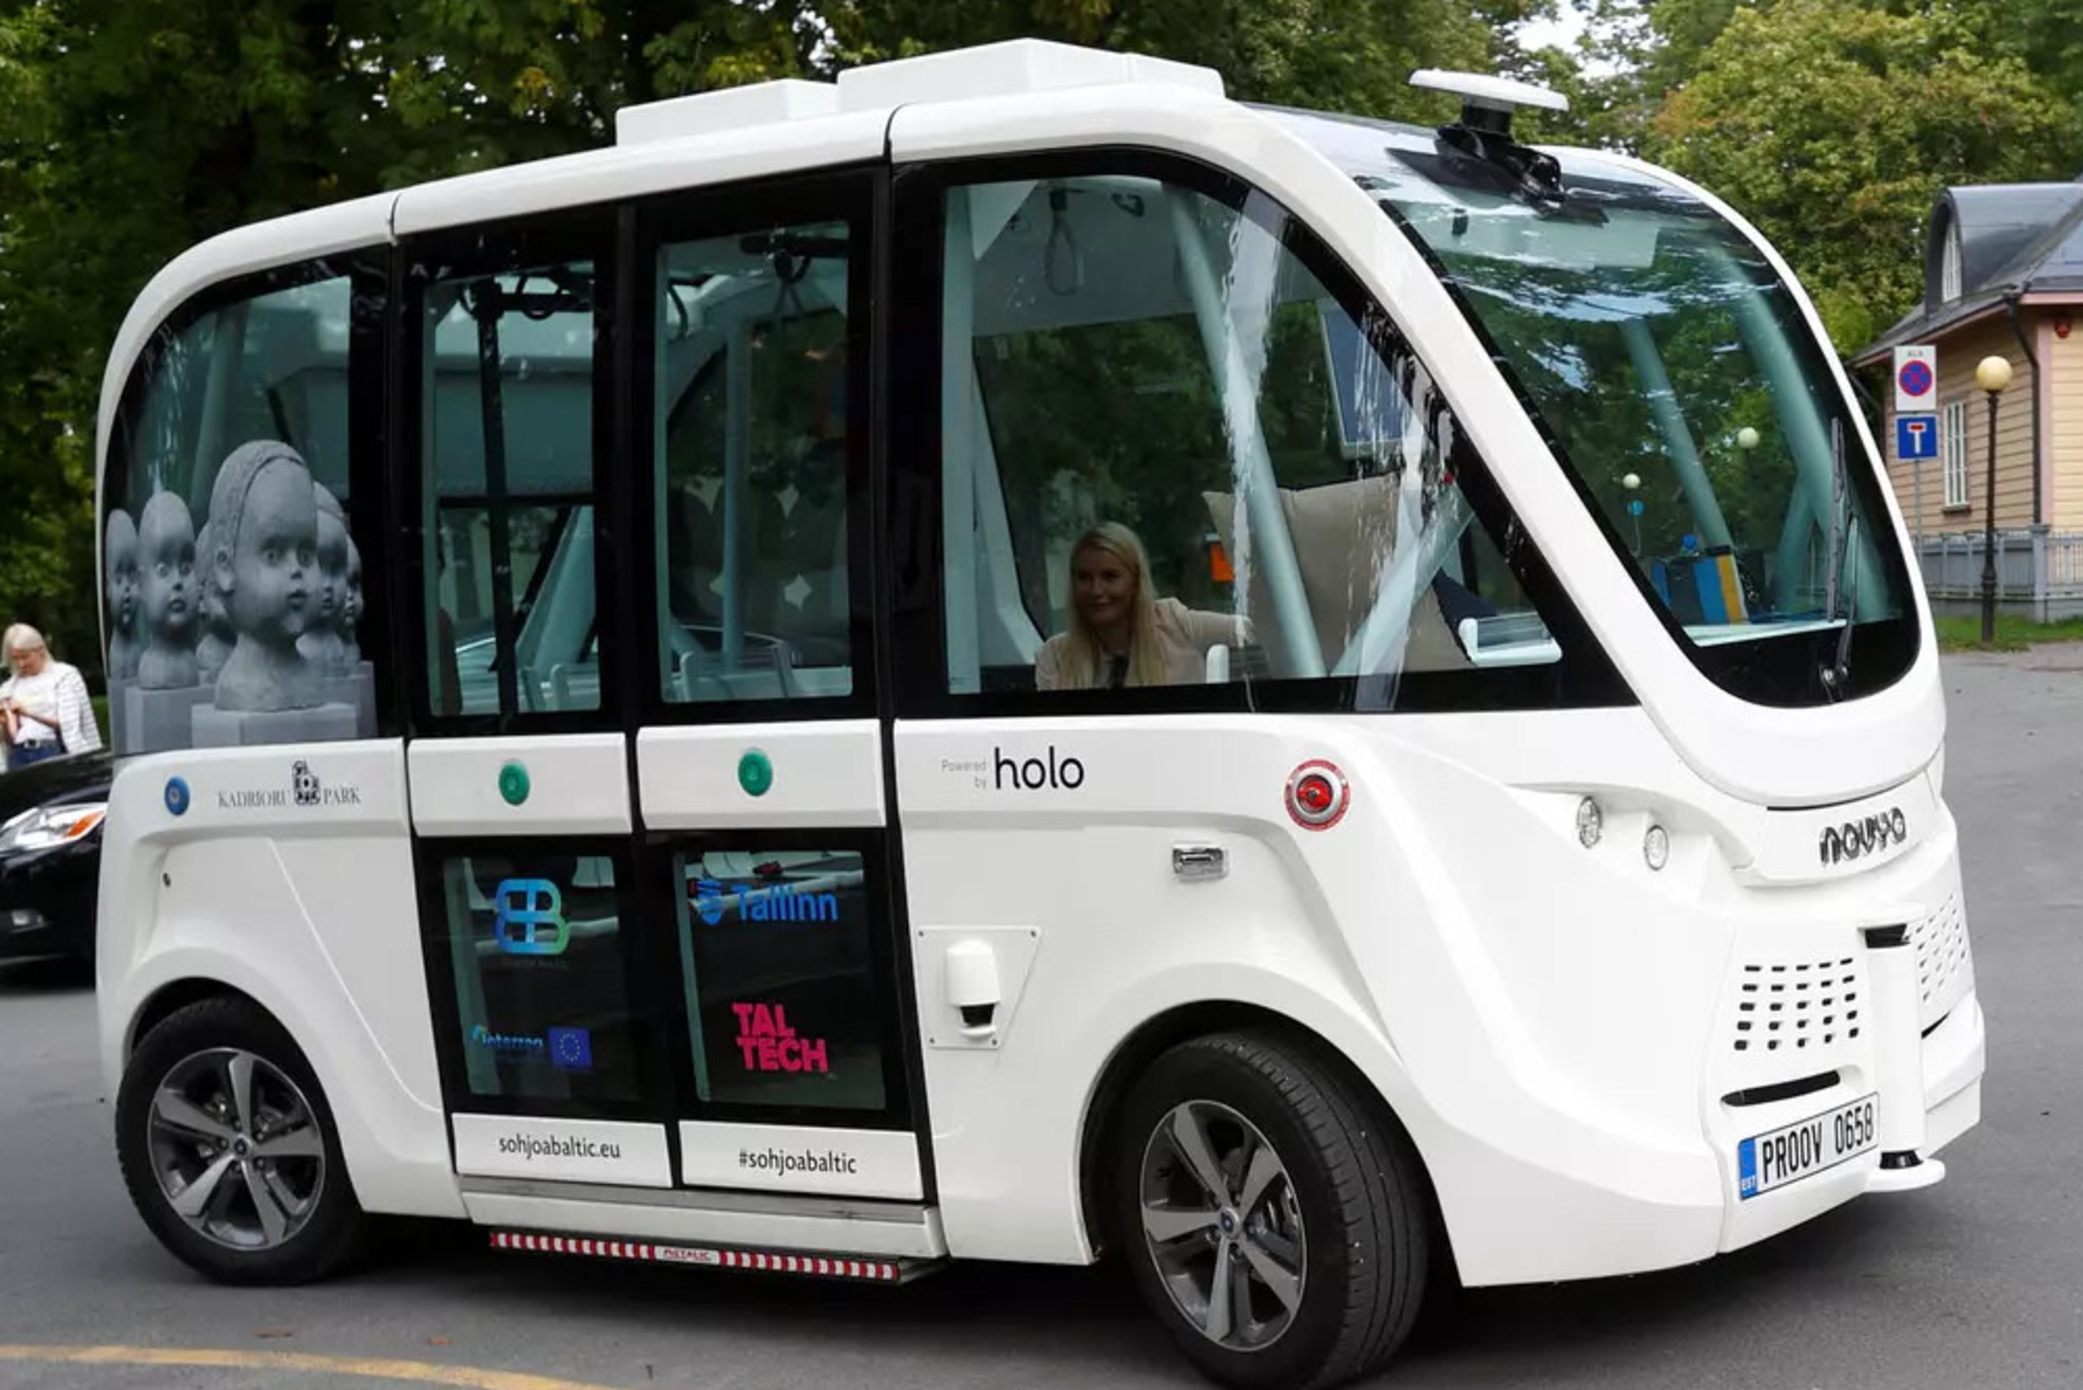
\includegraphics[width=\textwidth]{Apply1.pdf}
      \caption{无人驾驶公交车\cite{stephen2023driverless}}
      \label{fig:apply_sub1}
  \end{subfigure}
  \begin{subfigure}[b]{0.45\textwidth}
      \centering
      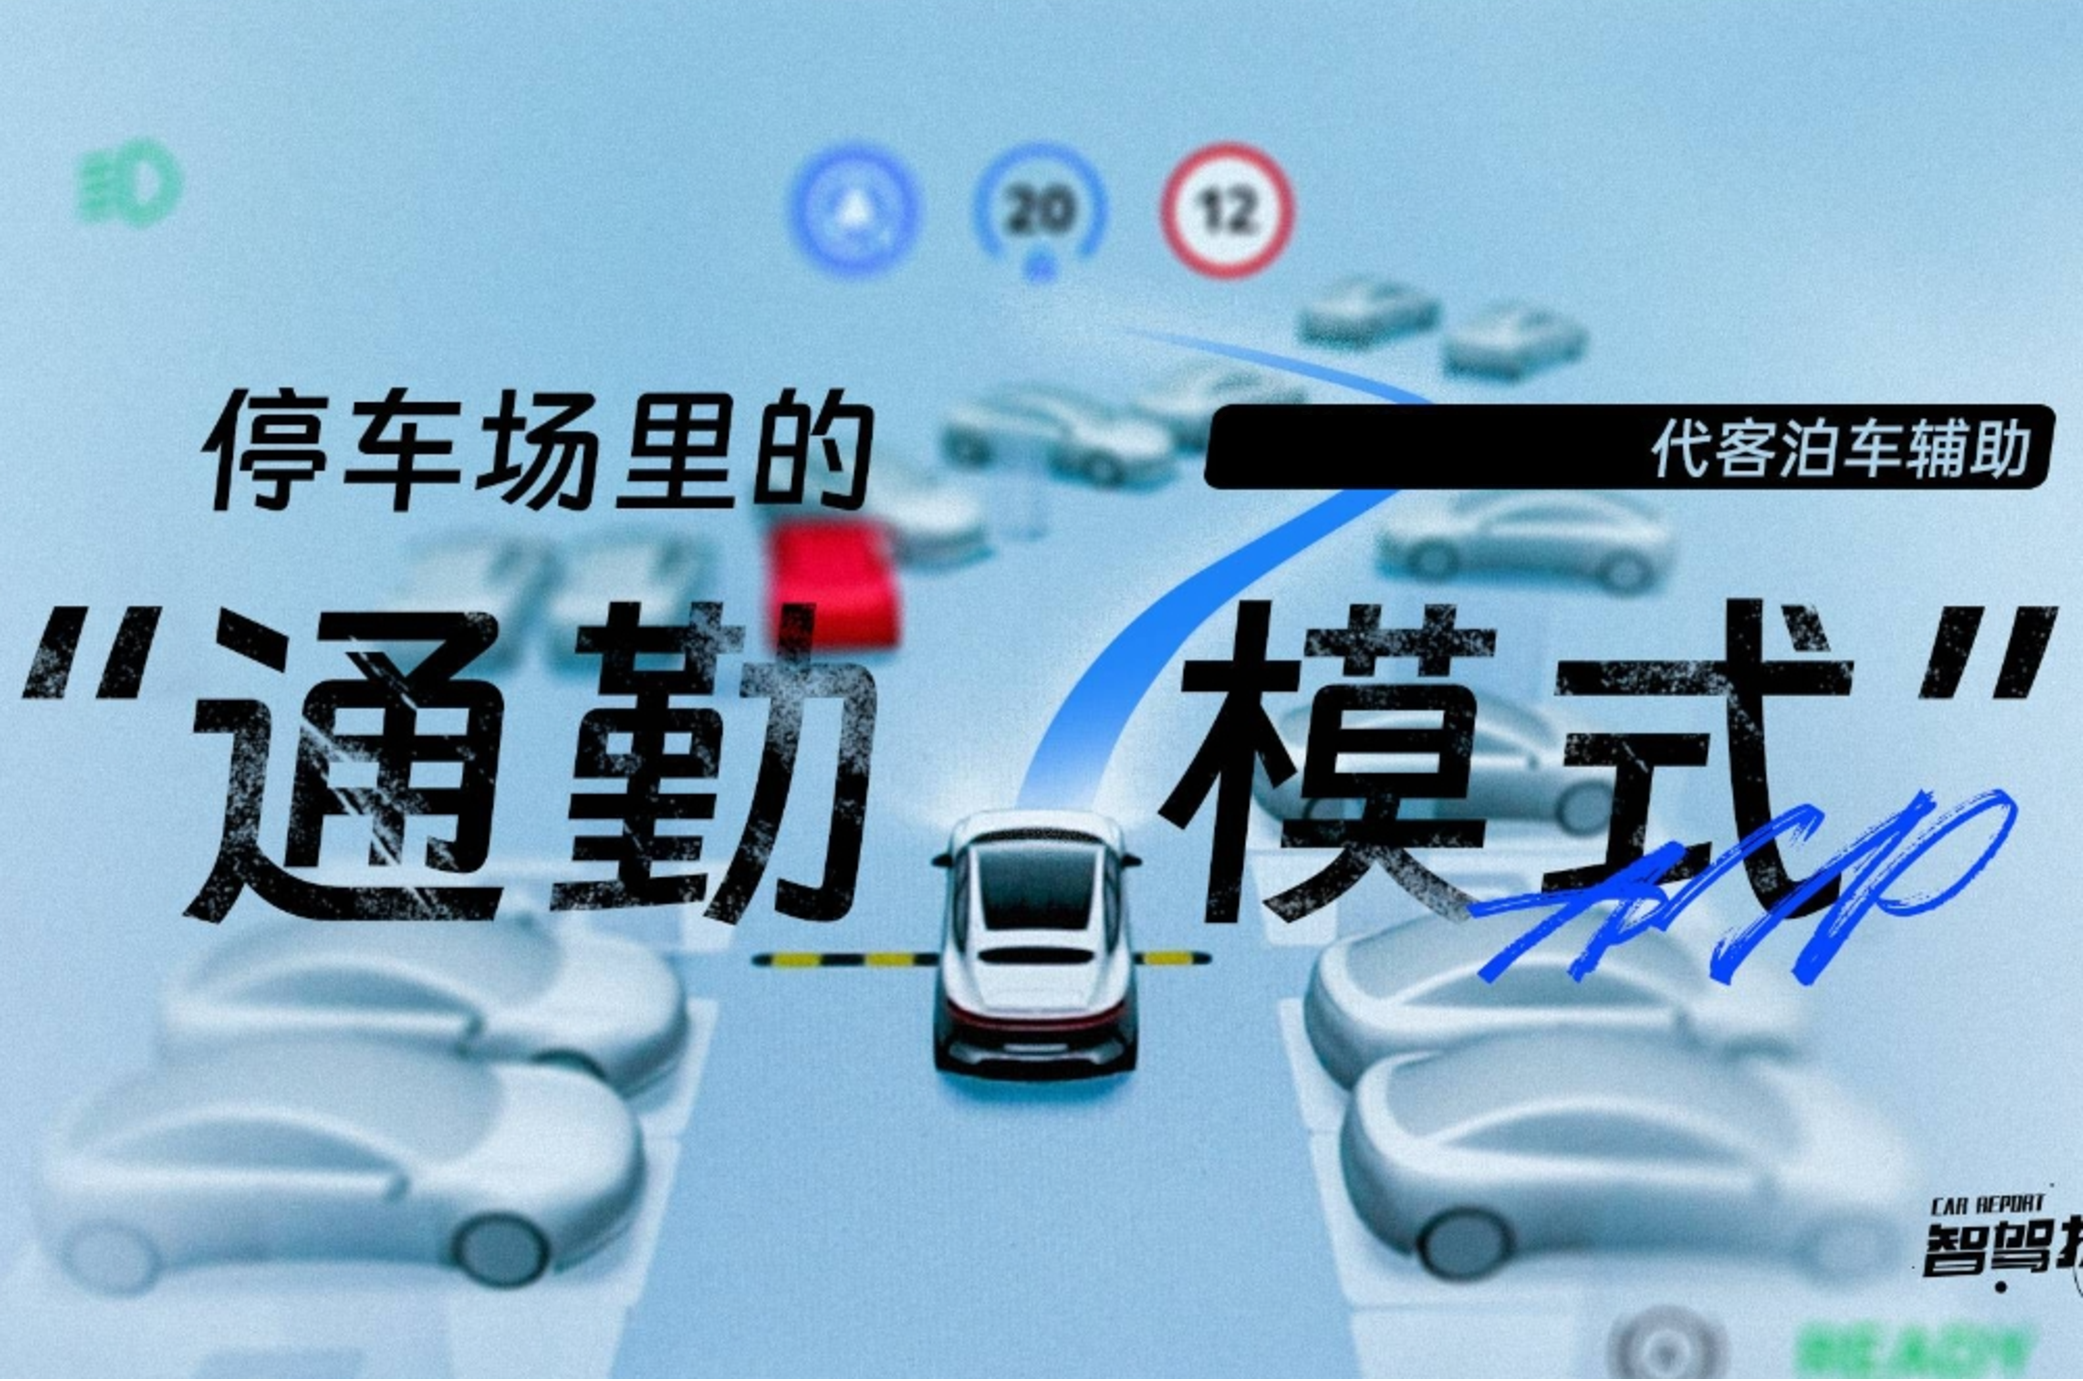
\includegraphics[width=\textwidth]{Apply2.pdf}
      \caption{智驾汽车通勤模式\cite{xin2023xinchuxing}}
      \label{fig:apply_sub2}
  \end{subfigure}
  \begin{subfigure}[b]{0.45\textwidth}
      \centering
      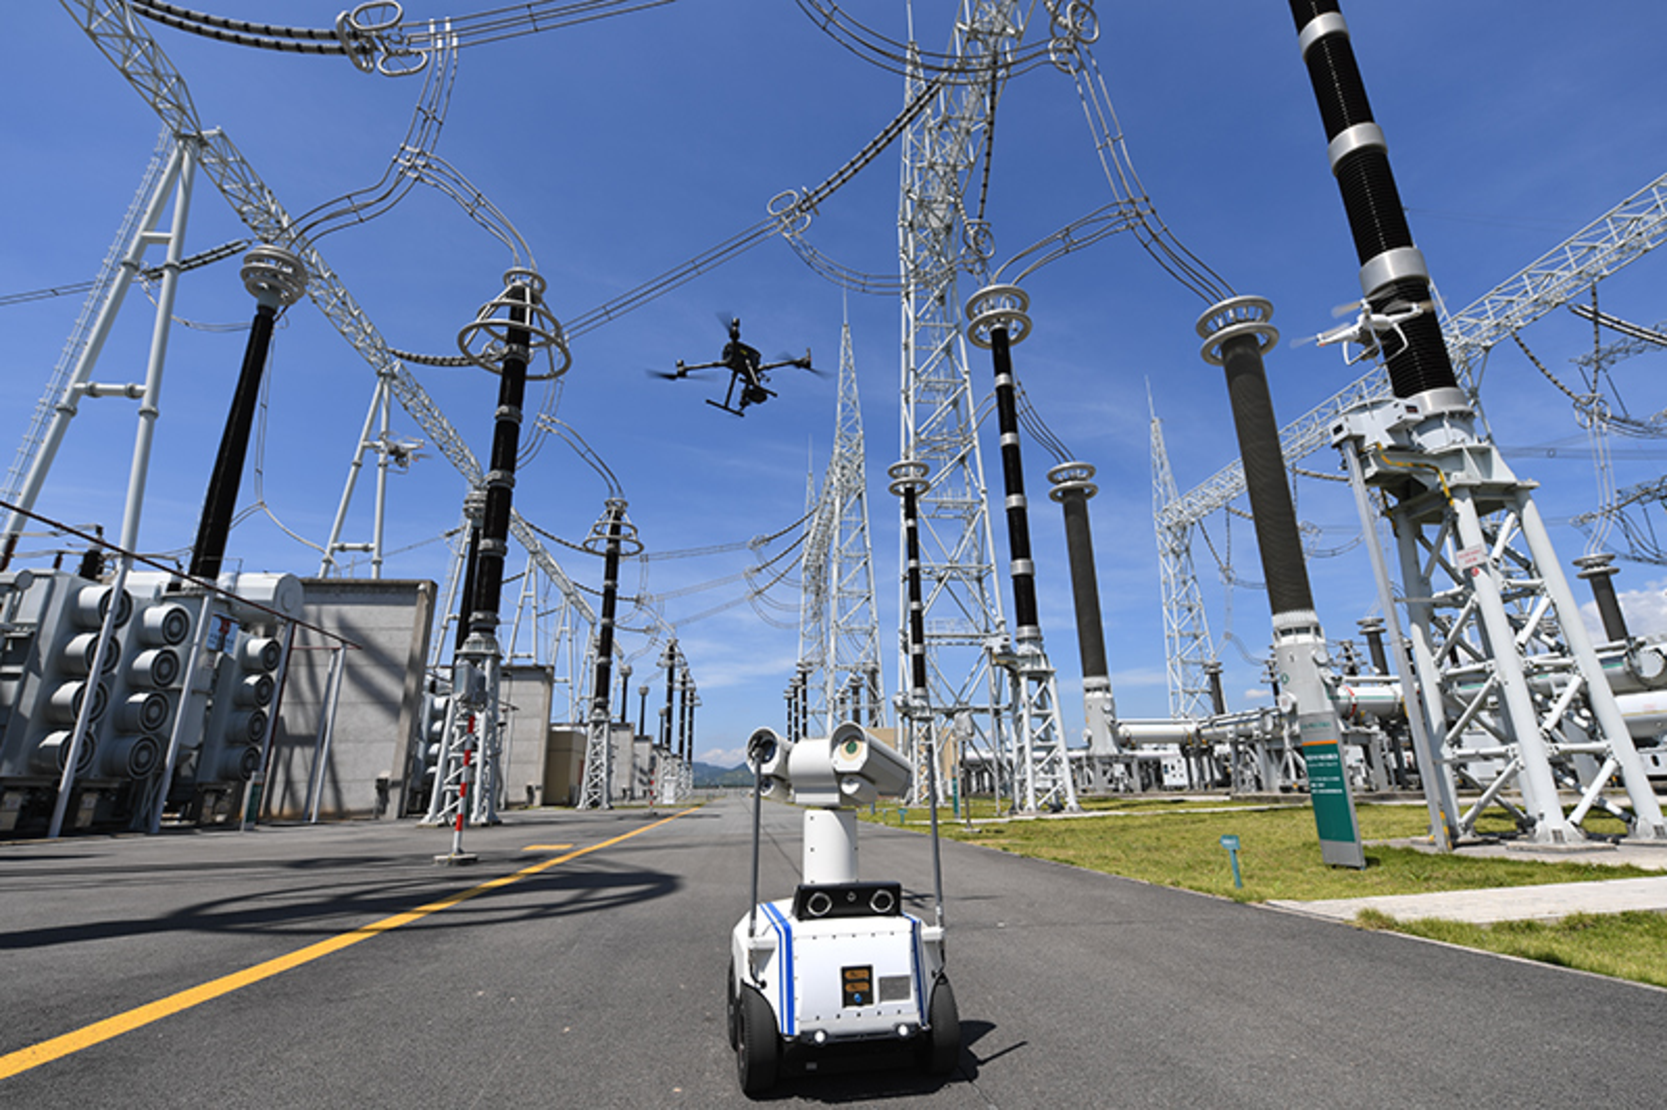
\includegraphics[width=\textwidth]{Apply3.pdf}
      \caption{变电站巡检车\cite{song2020xinhuawang}}
      \label{fig:apply_sub3}
  \end{subfigure}
  \begin{subfigure}[b]{0.45\textwidth}
      \centering
      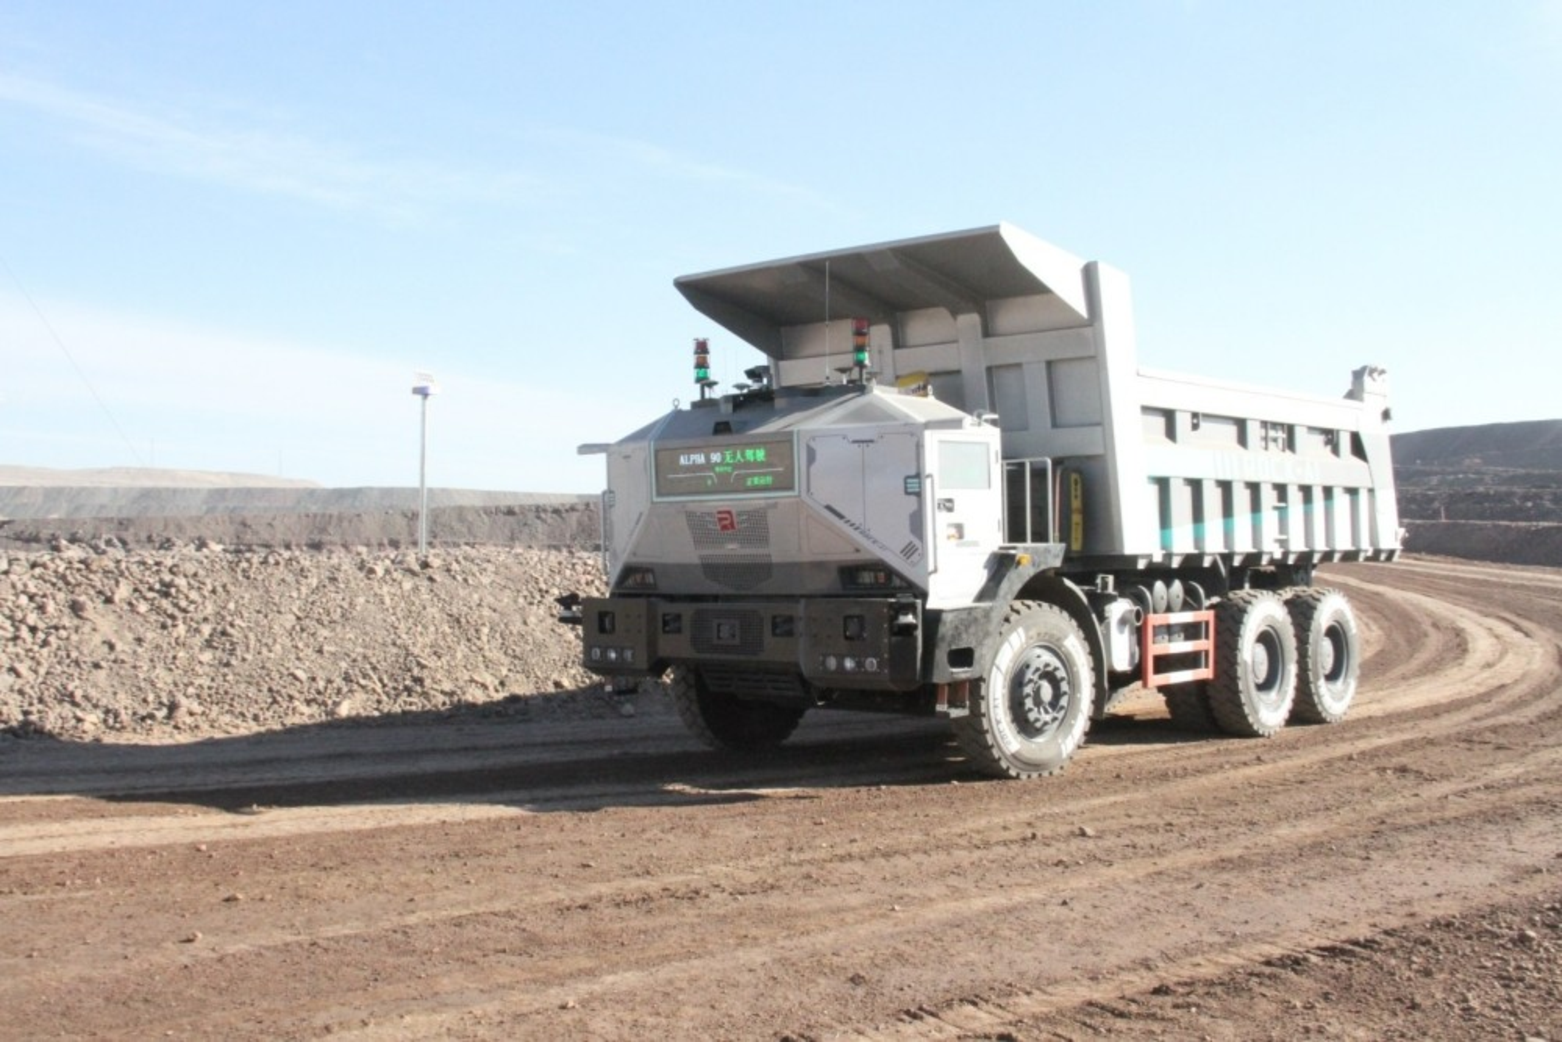
\includegraphics[width=\textwidth]{Apply4.pdf}
      \caption{矿山无人运输机器人\cite{li2023keji}}
      \label{fig:apply_sub4}
  \end{subfigure}

  \caption{固定路线智能体的应用场景}
  \label{fig:apply}
\end{figure}

在固定路线场景中,汽车和机器人运行在提前设置好的运行线路上,通过自身所具备感知能力对环境做出反馈,完成规划、导航等更复杂的任务。而在感知能力中,定位是十分基础但却十分关键的感知能力之一,定位系统是智能汽车和机器人运行的最基础系统之一。因此,固定路线中的精确定位是一项具有较高实用价值的基础性研究,只有实现了高精度的定位,才能确保复杂任务的可靠实施,才能保证整个智能体的安全。

在定位方法中,视觉惯性定位(Visual-Inertial Localization)是一种应用广泛的定位形式,它通过融合视觉和惯性传感器的数据,实现对自身姿态与位置的估计。视觉传感器可以获取环境的语义信息,而惯性传感器,例如惯性测量单元(Inertial Measurement Unit, IMU),可以获取自身的运动信息,两者结合可以实现对自身位置的估计。视觉惯性定位方法具有定位精度上限高、成本低、易于实现等优点,因此在固定路线定位中得到了广泛的应用。然而,视觉惯性定位方法也存在一些问题,例如视觉传感器易受光照、天气等环境因素影响,惯性传感器易受积分漂移等因素影响,这些因素都会影响视觉惯性定位的精度。因此,如何提高视觉惯性定位的精度,是当前固定路线定位研究的一个重要问题。

一种主要的改进方式是通过引入卫星导航系统(Global Navigation Satellite System, GNSS)信息来提高视觉惯性定位的精度。一般的商用低成本单频GNSS的精度在10米左右,这对于需要精确位置的智能化车辆和机器人来说是远远不够的。为了改进单频GNSS的精度,近年来出现了一些高精度的增强GNSS方法,例如精密单点定位(Precise Point Positioning, PPP)\cite{zumberge1997precise}技术和实时动态载波相位差分(Real Time Kinematic, RTK)\cite{fotopoulos2001overview}技术。PPP和RTK可以将GNSS的定位误差缩减至厘米级,是非常理想的高精度定位方法。但是PPP需要较长的初始化时间\cite{bisnath2018innovation},所以不适合应用在实时定位场景上。RTK虽然有不错的实时性,但是却经常容易受到天气、温度或者遮挡等问题的影响而产生单次误差较大的定位结果\cite{li2022review}。因此,直接引入GNSS观测信息会受到多种限制,并且高精度的GNSS服务也需要额外的费用,这对于一些低成本、大批量的固定路线应用来说是难以接受的。

\begin{figure}
  \centering
  \subcaptionbox{人类可理解语义地图\label{fig:sd_map}}{\includegraphics[width=0.45\linewidth]{SD_Map.png}}
  \subcaptionbox{视觉点云地图\label{fig:pc_map}}{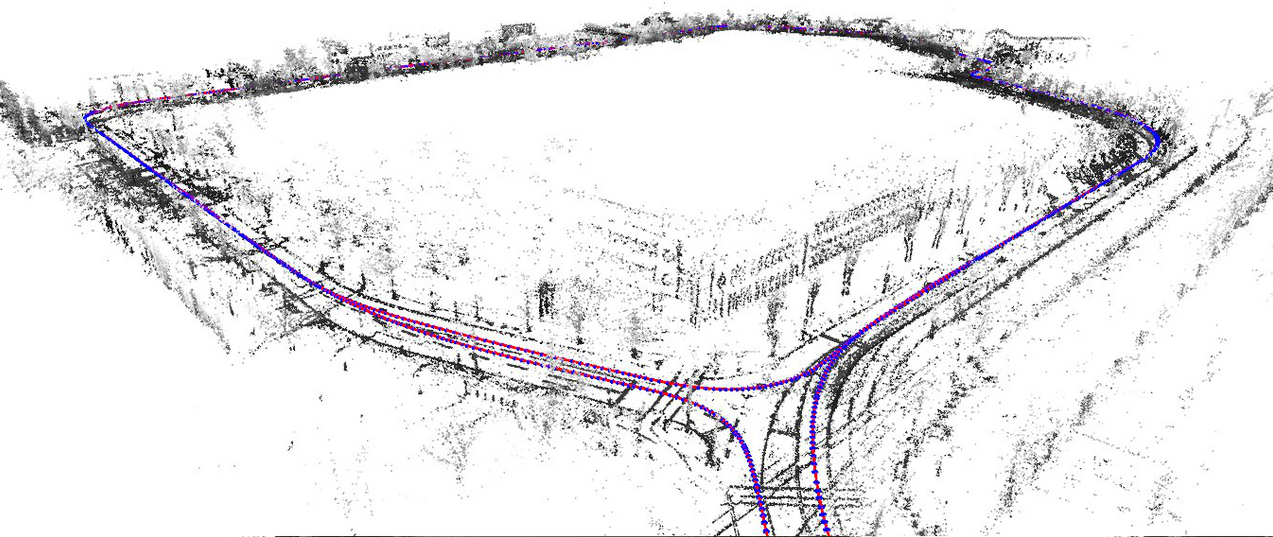
\includegraphics[width=0.45\linewidth]{sparse_pcmap.png}}
  \caption{不同类型的地图}
  \label{fig:maps}
\end{figure}

另一种改进方式是通过引入地图信息来提高视觉惯性定位的精度。此处所指的地图并非是人类理解的语义地图~\ref{fig:sd_map},而是稀疏点云地图,如图~\ref{fig:pc_map}所示。点云地图由图像、拍摄图像的相机位置与姿态,图像特征点及其空间坐标所构成,是一种适合计算机存储和使用的地图。地图信息可以提供给视觉惯性定位系统一个先验的位置信息,从而可以减小定位误差。在固定路线条件下,由于车辆或机器人运行的路线是固定的,因此可以提前获取到路线的地图信息,这方便于视觉惯性定位系统使用地图先验信息。除此之外,因为地图信息的收集过程没有实时性要求,可以在精心选择的条件下进行,所以还可以排除天气、温度等环境因素的干扰而使用高精度GNSS信息来辅助提高建图精度。从经济性方面考虑,先验地图可以一次建立、多次使用,而使用高精度GNSS往往需要购买连续运行参考站(Continuously Operating Reference Stations, CORS)服务商的持续服务\cite{CSKC202501011},会产生持续的运营成本。综合来看,引入地图信息有着较高的可实施性和经济性,是一种理想的提高固定路线视觉惯性定位精度的方法。

总的来说,固定路线中的视觉惯性定位是一项有着广泛应用的基础技术,但目前受限于视觉惯性定位技术本身的局限性,其精度还有待提高。在目前可选的改进方法中,引入地图信息是一种比较理想的提高视觉惯性定位精度的选择。因此,本文将围绕固定路线中的视觉惯性定位系统展开研究,通过解决地图构造、地图识别和地图使用等问题来提高定位的精度,设计一种精度满足需求,且具有实际操作性的固定路线中的视觉惯性定位系统。

\section{国内外研究现状}
\subsection{视觉惯性定位}

视觉惯性定位是一种融合了视觉、惯性信息的定位方法,其中视觉信息一般来源于图像、视频等,而惯性信息则一般依靠IMU采集。视觉惯性定位方法以视觉定位和惯性定位技术为基础,但是目前的视觉惯性定位技术一般以视觉定位技术为核心,而惯性定位技术作为补充或约束信息加入到视觉定位中,因此介绍视觉惯性定位的发展有必要从视觉定位技术的发展说起。

% \subsubsection[short]{视觉定位方法}

\begin{figure}
  \centering
  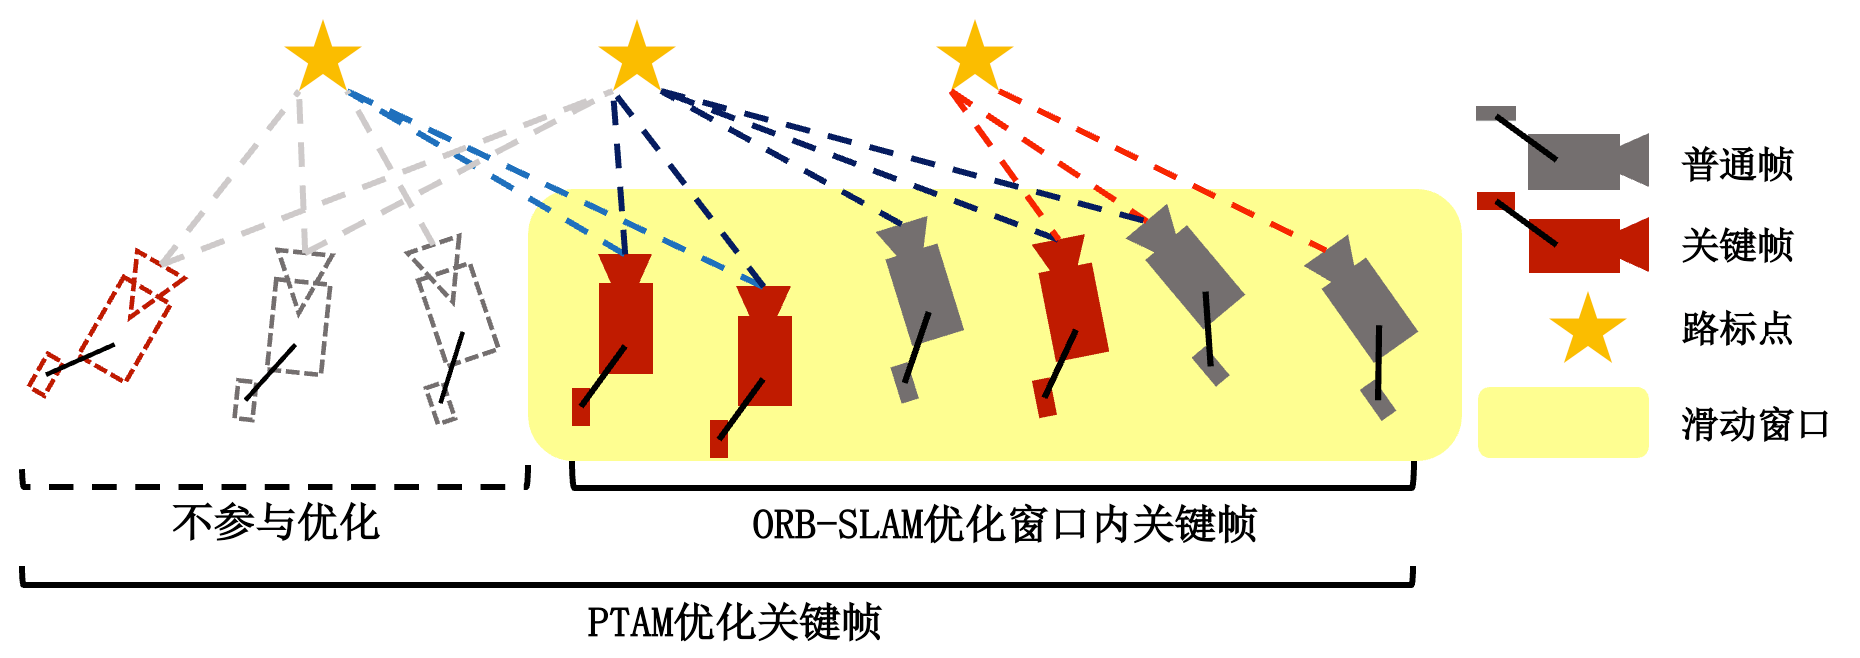
\includegraphics[width=0.9\linewidth]{vo_window.png}
  % \caption*{视觉定位中的关键帧和滑动窗口}
  \caption{视觉定位中的关键帧和滑动窗口}
  \label{fig:vo_window}
\end{figure}

视觉定位中常用的技术之一是同步定位与建图(Simultaneous Localization And Mapping, SLAM)。\citet{davison2007monoslam}于2007年首次提出了使用单目图像进行定位的方法MonoSLAM,以扩展卡尔曼滤波器(Extended Kalman Filter,EKF)为核心,实时对图像观测到的特征点进行位置估计,构建3D概率稀疏地图,然后使用地图点对相机位置和姿态进行估计,这是第一种能够达到实时的视觉定位方法,它使得利用视觉信息估计姿态成为可能。同年\citet{klein2007parallel}也提出了一种基于单目图像的定位方法PTAM(Parallel Tracking And Mapping) ,与MonoSLAM不同的是,PTAM的核心估计方法从扩展卡尔曼滤波器改变为光束法平差(Bundle Adjustment, BA)\cite{triggs2000bundle}。BA是一种非线性优化方法,其根据同一个地图点在多个图像上的观测位置,同时优化图像拍摄时相机的位姿和地图点的空间坐标。因为一次优化使用的数据更多,所以这种方法相比于滤波器更准确,但是计算量更大,所以PTAM引入了关键帧的概念:只对关键帧进行光束法平差,而对于普通帧则使用关键帧对其进行约束和定位估计。

PTAM 的另一大进步是将定位与建图两个功能解耦,使两个功能分别同时进行,而这一优点被\citet{mur2015orb,mur2017orb}吸取,创造出一个完整的SLAM系统:ORB-SLAM。ORB-SLAM包含3个主要线程:特征点实时跟踪(Tracking)线程、局部建图(Local Mapping)线程、回环检测(Loop Closing)线程。ORB-SLAM中不仅继承了PTAM的关键帧思想,还使用了如图\ref{fig:vo_window}所示的滑动窗口概念,进一步提高了系统实时性。滑动窗口设置包含固定数量关键帧的窗口,随着系统的工作,窗口随时添加新的关键帧并舍弃距离现在最远的关键帧,BA只优化当前窗口内关键帧及其地图点的信息。ORB-SLAM基本奠定了后来视觉定位方法的范式,其提出的3个功能模块也组成后续视觉定位方式的基本骨架。

虽然视觉定位的发展取得了一些进步,但是视觉定位的系统性缺陷却阻碍其应用。在视觉定位研究最广泛的单目视觉定位方面,其依靠的单目相机传感器天然缺少对深度的观测,这造成了单目视觉定位的尺度不确定性,即单目视觉定位不能获得真实世界尺度下的定位结果。为了解决这个问题,研究者们开始在视觉定位的基础上加入了可以获取真实世界尺度信息的传感器,例如惯性测量单元(Inertial measurement unit, IMU),提出了视觉惯性定位。

% \subsubsection{视觉惯性定位方法}
视觉惯性定位是视觉定位和惯性定位的结合,涉及到多传感器信息融合,根据融合方式可以分为松耦合\cite{lynen2013robust}与紧耦合\cite{falquez2016inertial}。松耦合方式是将视觉定位和惯性定位分开处理,让两种定位方式独立运行,然后对结果再进行融合,融合的方式可以选择扩展卡尔曼滤波或者非线性优化。松耦合的优点是系统简单,估计量少,因此不论是运行效率还是灵活度都非常高;缺点是忽略了两种定位方式之间的约束关系,所以精度较差。目前主流的视觉惯性定位基本是紧耦合方式,紧耦合需要将两种定位方式的估计量作为一个整体同时优化。

紧耦合视觉惯性定位方法最早以滤波器的形式发展,此时视觉惯性定位依旧是以IMU运动模型为核心,以线性化和观测性为主要研究方向,最突出的工作是\citet{mourikis2007multi}提出的多状态约束卡尔曼滤波(Multi-State Constraint Kalman Filter,MSCKF),该方法以IMU位置、姿态、速度等状态量和固定数量的相机位置、姿态为主要的估计参数,并没有将地图点加入到优化列表中。MSCKF工作的最主要贡献在于提出了一种能够表达从多个相机位姿观察到静态特征时出现的几何约束测量模型。

此后,许多基于MSCKF的工作相继提出,框架整体的精度和鲁棒性得到了不断的提升,例如\citet{li2013high}在MSCKF的基础上提出的MSCKF 2.0以及\citet{sun2018robust}提出的双目视觉版本MSCKF。\citet{bloesch2017iterated}提出了一种基于迭代扩展卡尔曼滤波器(Iterated extended Kalman filter,IEKF)的直接法单目视觉惯性里程计ROVIO(RObust Visual Inertial Odometry)。在视觉信息使用方面,ROVIO将地图点在图像中的观测点周围的图像块作为地图点的描述子,基于此图像块计算光度误差,然后以光度误差为基础构建IEKF中的启发项,进而进行滤波状态的更新。整体的滤波方程的构造是以IMU为中心进行构造的,保证能观状态不受不断增长的全局协方差的影响,这样可以减小因非线性而造成的误差。

\begin{figure}
  \centering
  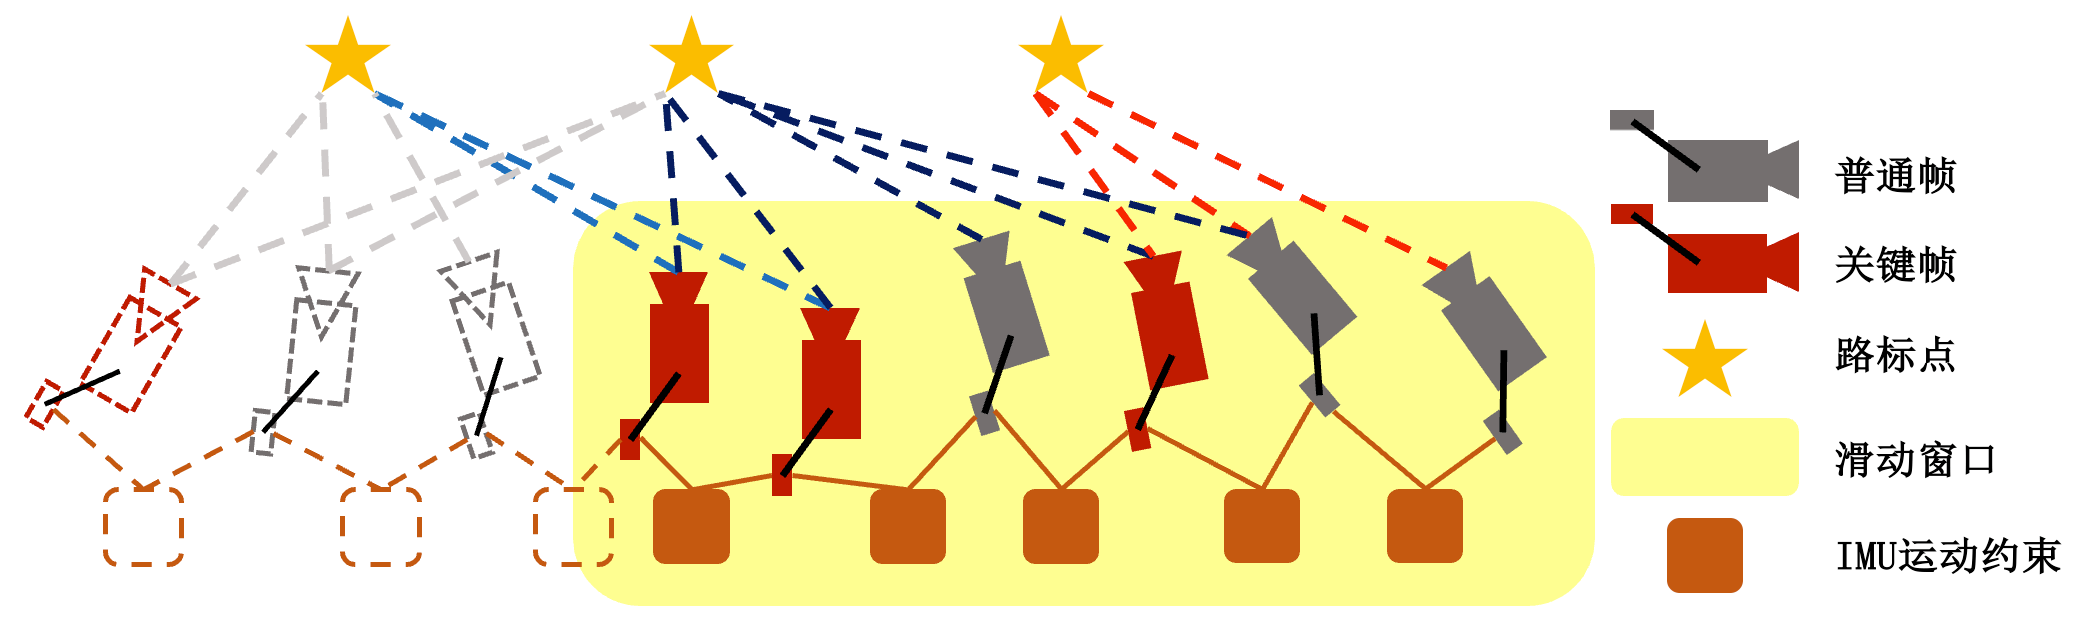
\includegraphics[width=1.0\linewidth]{vio_window.png}
  \caption{视觉惯性定位中的关键帧和滑动窗口}
  \label{fig:vio_window}
\end{figure}

近年来随着非线性优化在视觉定位中的广泛应用,视觉惯性定位方法也尝试使用这种优化方式。参考视觉定位中将地图点和相机位姿以图(Graph)的形式联系起来,然后使用光束法平差进行统一优化,视觉惯性定位在相机位姿之间加入由IMU数据组成的运动约束项,如图\ref{fig:vio_window}所示。IMU运动约束指的是IMU预积分,\citet{forster2016manifold}提出了应用于视觉惯性里程计中的基于四元数的预积分公式,将传统的IMU运动积分公式转化为帧间增量的形式,并且将运动积分中的IMU偏置(Bias)线性化,避免在优化过程中IMU偏置发生变化时重新积分,提高运行效率。\citet{leutenegger2015keyframe}提出的OKVIS(Open Keyframe-based Visual-Inertial SLAM)使用滑动窗口进行关键帧的批量非线性优化,滑动窗口之前的关键帧会被边缘化处理,不参与位姿估计。系统前端使用多尺度Harris\cite{harris1988combined}特征点和BRISK(Binary Robust Invariant Scalable Keypoint)\cite{leutenegger2011brisk}描述子构建帧与帧之间的数据关联。

\citet{qin2018vins}提出的VINS-Mono(Monocular Visual-INertial System)相较于OKVIS引入了几个全新的功能,包括观测值预处理、视觉惯性对齐初始化、局部视觉惯性优化、回环检测和全局位姿图优化5个部分,前端仍使用Harri特征点,但采用LK光流(Lucas-Kanade opticalflow)\cite{lucas1981iterative}法跟踪相邻帧之间的特征点。VINS-Mono 方法只计算特征点,不计算描述子,同时使用光流法跟踪特征点的运动,这样就减少了计算和匹配描述子的时间和资源。系统采用基于滑动窗口的紧耦合位姿估计方法,并且加入了基于词袋模型(Bag of Binary Words,DBoW)\cite{galvez2012bags}的回环检测线程,使系统具有重定位功能。\citet{liu2018ice}提出ICE-BA(Incremental, Consistent and Efficient Bundle Adjustment),沿用VINS-Mono中基于LK光流的特征点跟踪技术,后端则是提出了增量式BA,主要分为3个部分:局部BA、全局BA以及相对边缘化(Relative-Marginalization),局部BA、全局BA的使用提升了后端速度,相对边缘化保证了局部BA和全局BA的一致性。

一些视觉定位方法也发展出了融合惯性信息的版本,\citet{campos2021orb}在ORB-SLAM的基础上提出了ORB-SLAM 3,引入IMU尝试解决在快速运动时丢失特征点的问题:ORB-SLAM 3分别对ORB-SLAM的3个线程作出修改,用以融合IMU信息:在特征实时跟踪线程中,基于重投影误差和IMU预积分建立帧间的约束关系并构造代价函数,以代价函数为优化目标开展非线性优化从而得到位姿的最优估计;在局部建图线程中,当优化窗口中进入新的关键帧,将会只对窗口前N个关键帧进行优化,而新关键帧(第N+1帧)将被固定保持不变;在回环检测线程中,因为IMU观测提供了物理尺度信息,因此全局位姿图优化过程将从7自由度下降到6自由度,此外全局位姿图优化将忽略IMU所提供的帧间约束,即不再优化速度和IMU机械误差,当完成全局位姿优化后,再对速度进行修正。

\textbf{总结而言,视觉惯性定位系统的组成部分至今已基本定型,其主要由视觉SLAM系统的功能组件和预积分的惯性测量处理组成。因此,目前的视觉惯性定位方法仍遵循定位与建图同步的工作逻辑,并没有考虑过如何将先验地图运用到定位工作中。本文为了补充这一研究,希望提出一种地图辅助的视觉惯性定位方法,改变以往定位与建图高度同步的范式,这与此前的工作有较明显的差异。}

\subsection{地图辅助的定位方法}
地图辅助定位是一种车辆定位中常用的技术,常用的地图类型有高精(High-Definition,HD)地图、激光雷达点云地图、视觉重建地图等。\citet{jeong2020hdmi}开发了一种高效的HD地图表示方法,并利用粒子滤波器估计车辆的六自由度(6-Degree Of Freedom,DOF)位姿,该方法实现了分米级精度。\citet{xiao2020monocular}和\citet{guo2021coarse}提出了一种基于HD地图的低成本视觉定位方法。这两种方法综合利用了低级地图特征(如点和线特征)以及结构特征(如地图元素的语义和类别),从而能够精确估计车辆的位姿。尽管上述方法在定位方面取得了令人印象深刻的成果,但它们都依赖于成本高昂的高清地图,这些地图的构建需要细致的数据采集和人工标注。

为了降低对高清地图的依赖,研究者们开始探索基于图像和激光雷达扫描的地图构建方法。\citet{stewart2012laps}开发了一种利用单目相机在由搭载激光雷达传感器的测绘车辆预先生成的三维地图中进行定位的方法。该方法通过将激光雷达反射图像与图像强度进行匹配,并选择NMI(Normalized Mutual Information)最高的合成图像来确定相机位姿。\citet{zuo2019visual}采用基于MSCKF的视觉惯性里程计(Visual-Inertial Odometry, VIO)技术,在由激光雷达生成的点云地图中进行定位。具体而言,他们将点云地图作为观测值以更新MSCKF,从而提升其性能。\citet{lin2021autonomous}则将图像引入到先验地图信息中,其方法通过激光雷达估计位姿,同时利用车载图像构建稀疏点云地图。

近年来,随着视觉三维重建技术的进步,涌现了以SLAM和运动恢复结构(Structure from Motion,SfM)\cite{schonberger2016structure}为代表的地图重建方法。通过SLAM和SfM获得的重建地图一般包含地图关键帧的位姿、稀疏点云结构、稀疏点云特征等要素,这些要素可以在定位时快速提供粗略的位置参考,然后选择该位置附近的局部点云地图与当前定位图像进行细匹配和优化定位。具体来说,重建地图的地图关键帧的位姿可以通过特征点匹配、局部地图优化和全局地图优化等手段获得;重建地图的稀疏点云结构一般是通过提取地图关键帧的特征点,并根据地图关键帧的相对位姿三角化获得;重建地图的稀疏点云特征则是由地图关键帧的特征点描述子组成。在定位过程中,首先将待定位图像的特征点与地图的稀疏点云进行匹配,匹配到足够的地图点后可以使用PnP(Perspective-n-Point)算法直接计算待定位图像的位置和姿态。

在具体的重建地图使用方面,VINS-Mono、VINS-Fusion和ORB-SLAM 3等一些SLAM系统都已具有保存和加载先验地图的功能,这些SLAM系统可以提前在指定场景下初始运行、建图,而在此后的运行中依靠初始运行的结果进行定位。\citet{surber2017robust}提出了一种针对无人机的定位系统,旨在利用相机和IMU,在初始飞行中构建参考地图。在后续飞行中,系统通过VIO和图像匹配技术,将当前观测与参考地图进行对比,实现精确的自我定位。\citet{hao2023global}提出了一种两阶段的视觉惯性定位系统:在初始运行的过程中加入了额外的GNSS信息建图,而在后续运行中保持纯净的视觉惯性定位。在此系统中,初始运行阶段的GNSS信息提供了较强的位置约束,因此其所建地图精度得到了提升。这些地图使用方法思考了如何建立先验地图和实时场景中的特征点匹配关系,从而使用先验地图的精确地图点为当前定位提供参考。

然而,上述方法在匹配过程中依旧使用着传统的手工设计特征,这些特征在匹配精度和鲁棒性上仍有提升空间。除此之外,上述方法的重建地图基本都是基于SLAM系统的,这意味着地图的构建和定位是高度耦合的,系统本身的建图误差会传导、积累到定位过程中。虽然有工作\cite{hao2023global}尝试在建图阶段加入额外位置信息,提升建图效果,但其仍使用注重实时性的SLAM系统进行建图,依然会受到SLAM系统误差累积的影响。为了提升特征匹配的精度,同时降低建图误差对定位的影响,一些研究者开始尝试使用基于深度学习的特征搭配精度较高建图技术,例如SfM或者带GNSS增强的SfM\cite{vincentqin2022colmapgps},来提升整体的定位精度。

\citet{sarlin2019coarse}提出了一种“由粗到细”的地图使用方式:其建图过程使用SfM和具有精确位姿的图片进行;其定位方法首先使用基于深度学习的图片级描述子NetVLAD(Vector of Locally Aggregated Descriptors)\cite{arandjelovic2016netvlad}对定位图片进行粗位置查询,此后使用基于深度学习的像素级描述子SuperPoint\cite{detone2018superpoint}对定位图片的特征点进行细致匹配。这种方法在匹配过程中使用了基于深度学习的特征,从而提升了匹配的精度和鲁棒性,同时具有较高的实时性,为后续许多工作提供了一种地图定位范式。\citet{yang2022real}提出了一种基于视觉重建地图的定位方法,其方法在“由粗到细”定位的基础上引入了VIO,利用实际定位中的帧间相对位姿约束提升了定位精度。\citet{lin2023visual}则更是引入了多地图概念,其方法在匹配过程中使用了多个地图,从而提升了匹配的鲁棒性。近年来,由于深度学习端到端技术的启发,也出现了一些使用隐式地图使用的定位方法,\citet{xue2020learning}提出的GNNMapNet与\citet{wang2023robustloc}所提出的RobustLoc都是这类方法的代表。这类方法使用带有坐标和姿态的图像作为训练集进行训练,在推理时可以只输入图像就端到端地输出定位结果。

\begin{figure}
  \centering
  \subcaptionbox*{GNNMapNet\cite{xue2020learning}定位(红色)效果\label{fig:gnnmapnet}}{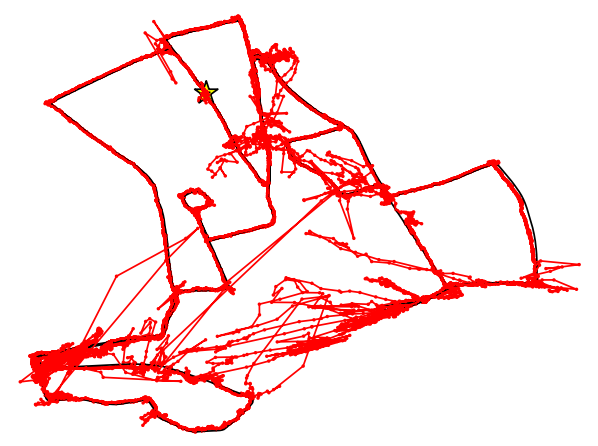
\includegraphics[width=0.45\linewidth]{gnnmapnet.png}}
  \subcaptionbox*{RobustLoc\cite{wang2023robustloc}定位(红色)效果\label{fig:robustloc}}{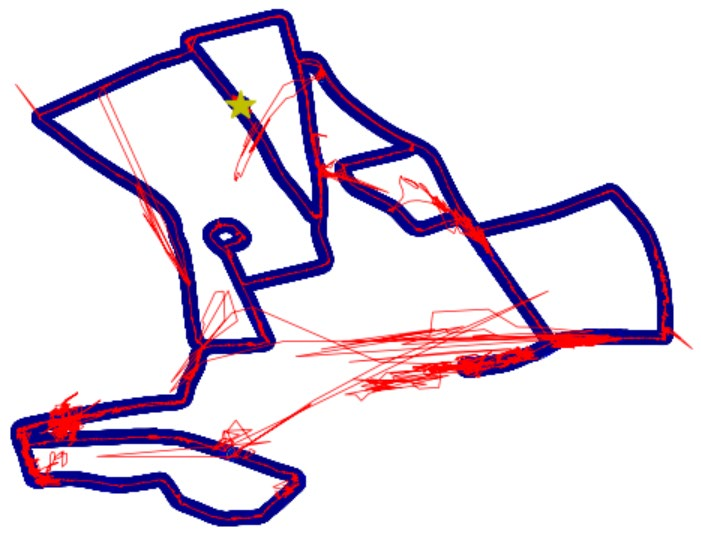
\includegraphics[width=0.45\linewidth]{RobustLoc.png}}
  \caption{端到端定位效果}
  \label{fig:e2eloc}
\end{figure}

虽然这些方法在最终的定位精度上有所提升,但是存在一些问题。首先,这些研究在建图时直接假设地图图片的准确位姿是可获得的,这在实际操作中并不一定总是成立的。其次,这些研究聚焦于先验地图和实际定位之间的匹配关系,并尝试通过各种手段来增加匹配的约束,例如相对位姿、多地图验证等,但是却并没有考虑当地图和定位场景之间产生误匹配时如何降低误匹配的影响。这无疑导致了这些定位方法的脆弱性,使得他们在实际应用中表现出不稳定的性能。此外,\citet{yang2022real}在定位中引入了服务器组件,因此对通信环境的要求较高;\citet{lin2023visual}的方法使用多地图以及丰富的约束,导致运行过程内存占用极大(测试中使用4T RAM);GNNMapNet和RobustLoc这类端到端的定位方法表现极不稳定,产生的轨迹平滑性不足,如图~\ref{fig:e2eloc} 所示。这些问题都限制了上述方法在实际应用中的推广。

\textbf{总结而言,地图辅助的定位方法研究较为分散,根据地图类型的不同,定位方法差异较大。使用HD地图和激光雷达点云地图的方法有较高精度,但是高昂的地图成本却也阻碍着这类技术在实际生产中的应用。基于重建地图的定位方式有较低的成本,但是当前的研究方法中还有一些限制,例如建图假设过强、定位容错不足和实际应用限制较多等问题。为了提供一种实施难度低、容错能力强、完全部署在汽车或机器人上的高精度定位方法,本文希望从建图方式开始,构建完整的固定路线中的视觉惯性定位系统,实现完全部署于车载或机器人端,并具有较高定位精度。}

% \section{研究意义}

% (1) 以视觉惯性定位为基础,引入地图信息提高定位精度,是当下一种较为新颖的定位技术,本文以实现这一技术为目标,提出一种完整的固定路线视觉惯性定位系统设计,为这一技术的研究提供了一种新的思路,具有一定的理论意义。

% (2) 固定路线中视觉惯性定位系统的实现使用了多传感器信息融合,状态实时估计等多种技术,将多种技术合理得设计到一个整体中,实时准确得完成定位任务,对推动固定路线中的智能汽车和机器人技术发展具有实践意义。

% (3) 本文在地图的构建和使用中不仅有传统的空间计算、状态估计和非线性优化技术,还引入了基于深度学习的计算机视觉技术,对于推动传统定位技术和深度学习技术的融合具有一定的实践意义。


\section{研究内容}

本文的研究内容是设计一种完整的固定路线视觉惯性定位系统,具体而言,本文将通过设计3个子模块分别解决“高精度先验地图构建问题”、“符合车辆运动学的视觉惯性融合问题”以及“地图观测与定位优化问题”,此后将3个模块整合到一起,形成一个完整的固定路线视觉惯性定位系统。

\subsection{解决高精度先验地图构建问题}

先验地图的构建是本文首先要解决的问题,是剩余其他研究内容的基础。因为SLAM类建图算法有实时运算要求,因此只能进行局部优化,所以存在误差累积,精度较差的问题。为解决这一问题,本文采用SfM作为基础建图方法,其全局优化策略可以有效降低累计误差。

虽然SfM建图具有理论精度高的优势,但原始的SfM建图不具备现实尺度。为了恢复出具有现实世界尺度的地图,必须增加有现实尺度的观测信息,本文所采用的观测信息为高精度GNSS(例如RTK)观测。虽然RTK在使用时可能会存在瞬时测量受环境因素影响而产生波动等问题,但是对于建图环节来说,环境可以静心挑选,因此RTK完全可以运用在实际建图中,并且其较高精度的定位观测可以为建图优化提供较好的约束。

本文将着力于融合GNSS观测信息与SfM,提出一种精度较高且稳定性突出的视觉先验地图构建方式,所构建的地图将具有现实世界尺度,且地图关键帧具有较高的位姿估计精度,以此来解决先验地图构建问题。

\subsection{解决符合车辆运动学的视觉惯性融合问题}

视觉惯性信息的融合是定位的核心步骤,融合的好坏决定着最终定位的精度。目前视觉惯性信息的融合方式主要分为卡尔曼滤波器和非线性优化两种,其中卡尔曼滤波器的优势是在估计矩阵维度较低时计算简单,速度较快,劣势是精度欠缺;非线性优化的方法能够提供较高的精度,且随着硬件技术进步,实时运行非线性优化方法也是可能的。

当下基于非线性优化的视觉惯性融合方法,大多数优先考虑通用场景,对于固定路线中运行的车辆或轮式机器人缺乏特殊设计。车辆和轮式机器人的运动有其特有的规律和约束,通用的设计往往难以满足这些约束,导致估计的车身状态有时会与车辆运动学产生明显冲突,例如会在车身横向和重力方向产生持续速度估计误差,这种冲突也降低了状态估计的精度。

本文选择以非线性优化作为融合方案,着力于解决如何在非线性优化中构建视觉信息和惯性信息的约束关系,并加入符合固定路线运行的车辆和机器人车辆运动学的合理约束,提高融合后的状态估计精度。

\subsection{解决地图观测与定位优化问题}

地图观测与定位优化是将先验地图与实际定位过程结合的关键。地图观测首先要解决的问题是将地图点与待定位图像特征点进行关联,构建图像特征点观测与图像位置、姿态参数之间的转换关系。基于特征点和描述子的关联方式具有一定的可行性,但是考虑到建图过程可能与实际定位过程有较大的场景表现差异,需要选择对场景差异不敏感的特征点及描述子。

定位优化是获得高质量定位结果的必要步骤,由于地图观测中的各种误差,定位结果通常表现为不稳定的状态,为了维护一个相对稳定、平滑的轨迹,需要定位优化过程。在本文的系统中,视觉惯性融合的结果能够提供较为精确的帧间相对位姿,再结合对地图的观测,可以进一步提高定位精度。但是如何处理两种来源(地图观测与视觉惯性融合)的信息,如何处理两种来源信息的内在误差,是需要解决的问题。

本文将着力于使用一种基于数据驱动的,能够对场景差异较为鲁棒的先验地图观测技术,构建定位与先验地图的关联。在此基础上使用一种考虑多种误差的定位优化方法,将地图观测与视觉惯性融合的结果进行优化,以获得高精度的定位结果。

\section{研究创新点}
本文的创新点主要体现在以下几个方面:

(1) 提出了一种新颖且完整的固定路线视觉惯性定位方法,该方法将“高精度先验地图构建”、“符合车辆运动学的视觉惯性融合”、“地图观测与定位优化”三个内容有机结合,形成一个完整的视觉惯性定位系统。

(2)在高精度先验地图构建方面,本文提出了一种融合SfM与GNSS的离线建图模块,采用SfM和高精度GNSS观测数据相结合的方式,构建具有现实世界尺度的多层次先验地图,提高地图的精度和稳定性。

(3)在符合车辆运动学的视觉惯性融合方面,本文提出了一种基于车身运动模式感知的伪观测视觉惯性里程计(Pseudo Obsevation Visual-Inertial Odometry, PO-VIO),该VIO使用深度神经网络对车身运动模式进行检测,针对直行状态下的车辆或轮式机器人进行速度观测约束,提高了里程计的估计精度。

(4)在地图观测与定位优化方面,本文在模块设计中使用了基于深度学习的地图特征来完成地图观测,数据驱动的特征相较于传统手工设计特征能更好适应变化场景。基于最大后验概率估计的定位优化方法,将地图观测与视觉惯性融合的结果进行优化,同时引入了地图点的误差建模,获得了高精度的定位结果。

\section{固定路线中的视觉惯性定位系统整体设计}

本文所提出方法的整体系统设计如图~\ref{fig:overall} 所示,其主要包含3个模块:离线建图模块、PO-VIO模块和地图定位模块。在3个模块中,离线建图模块负责构建先验地图;PO-VIO模块和地图定位模块负责实际定位。PO-VIO使用图片和惯性信息可以获得连续图片的相对位姿变换;地图定位则使用视觉惯性里程计结果和地图观测完成最后的定位,获得相机位姿。整个系统的设计与研究内容的对应关系是:离线建图模块对应着解决高精度先验地图构建问题的研究内容,PO-VIO模块对应着解决符合车辆运动学的视觉惯性融合问题的研究内容,地图定位模块对应着解决地图观测与定位优化问题的研究内容。

\begin{figure}
  \centering
  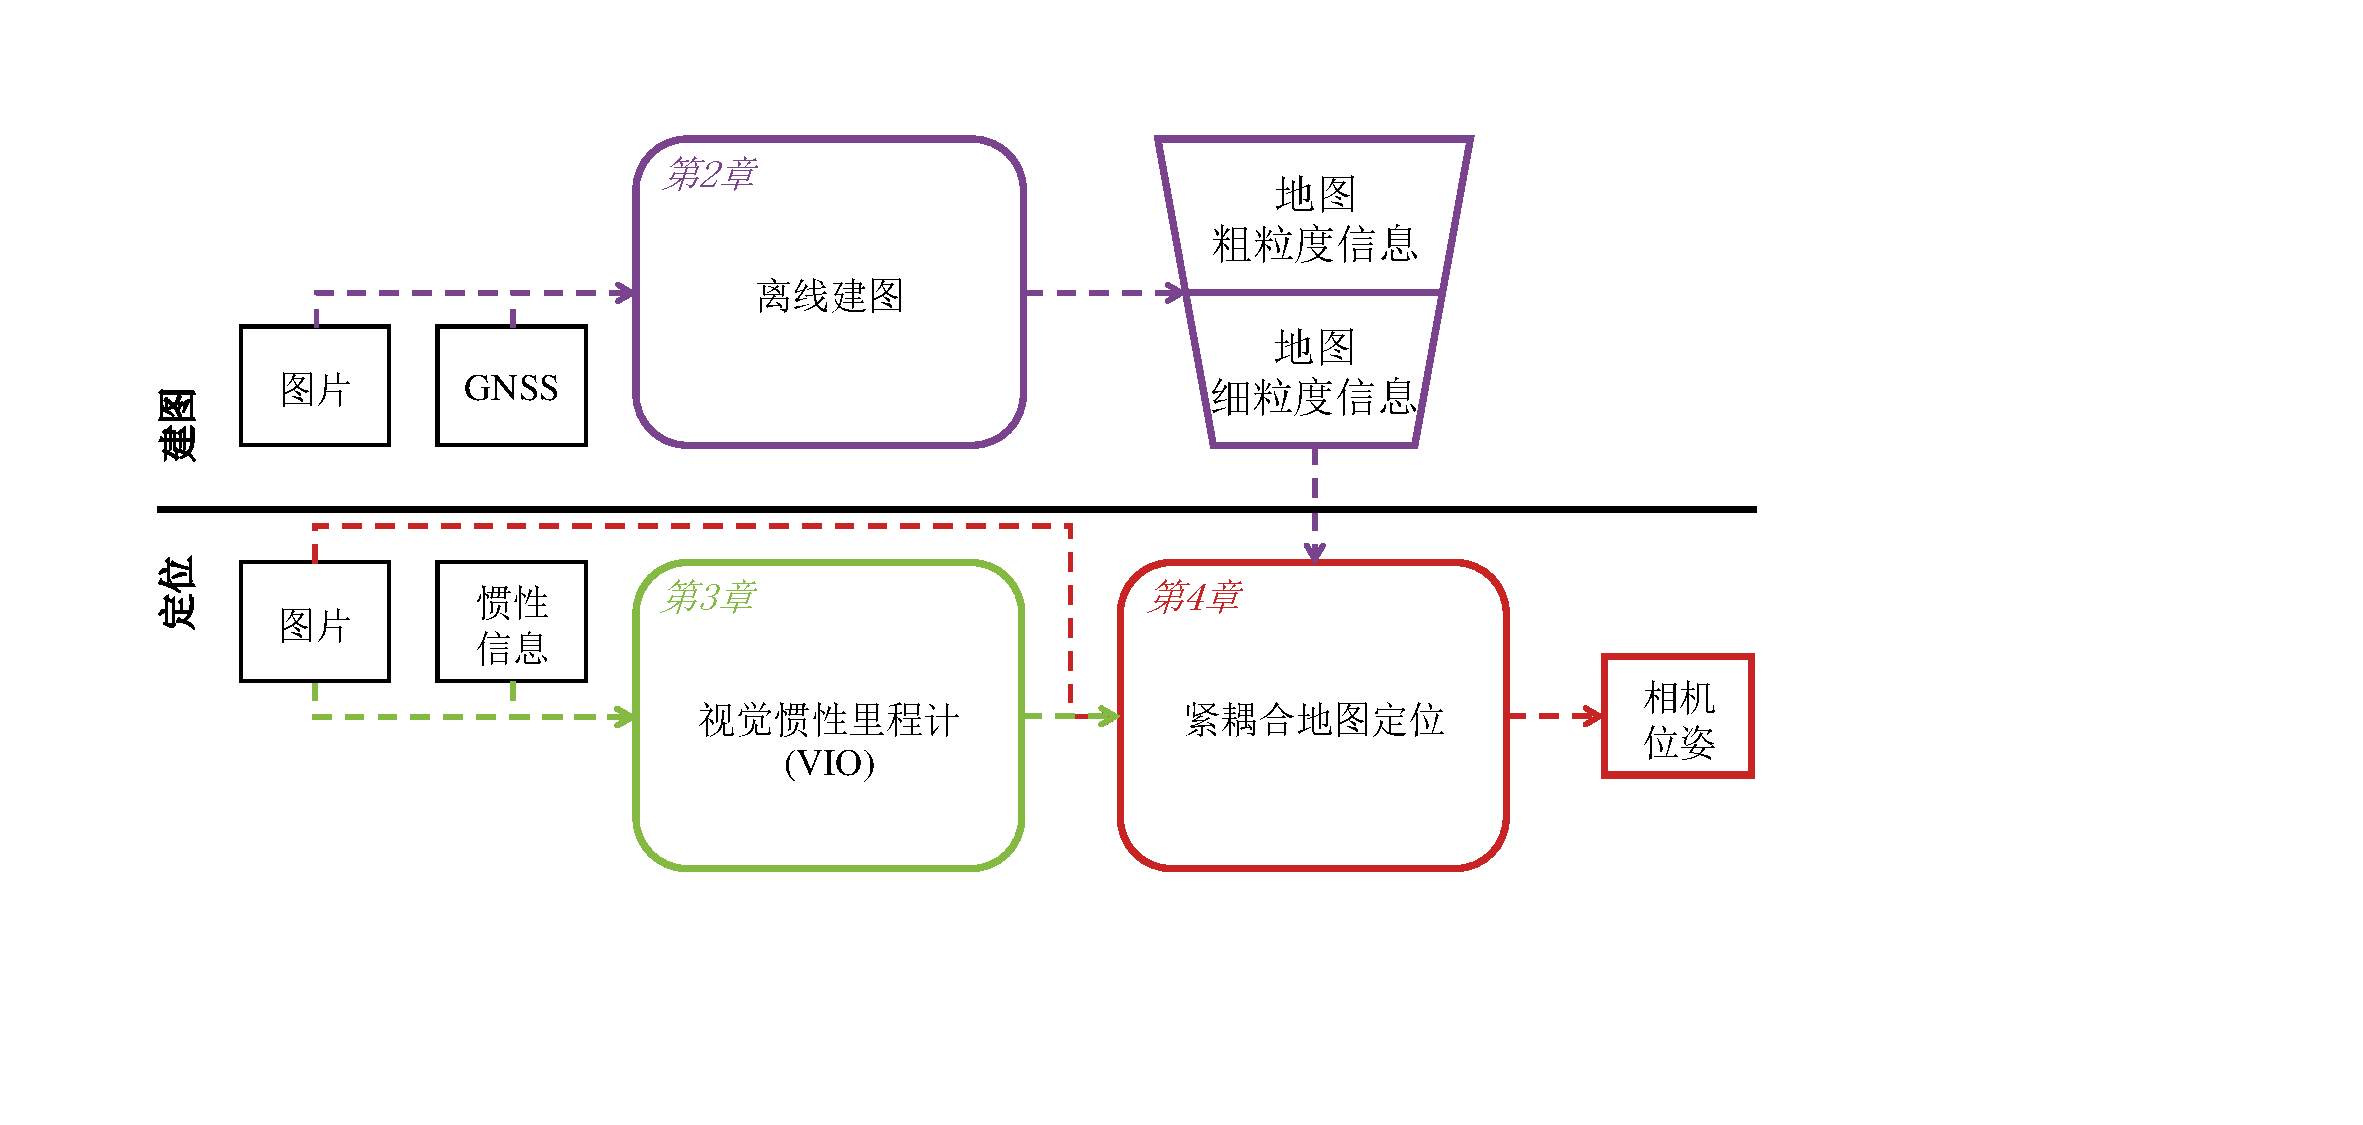
\includegraphics[width=1.0\linewidth]{overall.pdf}
  \caption{系统整体设计示意图}
  \label{fig:overall}
\end{figure}

离线建图模块利用GNSS观测数据和图像构建一个包含粗粒度层级和细粒度层级组成的分层先验地图。粗粒度层级包括地图关键帧的位姿和关键帧描述子,而细粒度层级则包含稀疏点云结构及点云点描述子。

GNSS增强的SfM是离线建图模块的核心,使用这一技术有以下的必要性:首先,SfM作为一种具有全局优化功能的建图方式,其相较于SLAM更适合建立高精度的地图;其次,SfM作为一种单目建图技术,其所创建的地图并不具有真实物理世界的尺度,因此必须添加具有尺度信息的GNSS信息作为补充,以获得具有真实世界尺度的地图;最后,相对精确的GNSS信息对于SfM的建图过程也有增益,有助于获得更加精确的地图。

基于分层先验地图,PO-VIO模块和地图定位模块计算实际定位时所拍摄图像在全局坐标系中的位姿。

在PO-VIO模块中,图像和惯性信息经过融合后可以相对精确地估算相邻图片之间的位姿变换,虽然相对位姿不可以直接用来作为定位结果,但是可以作为约束条件用于实际的地图定位。作为一种约束条件,视觉惯性里程计的精度对于整个定位系统的性能也发挥着重要作用,因此,本文根据车身运动学的合理假设提出了基于车身运动模式感知的PO-VIO模块设计:车身的运动模式可以在不增加传感器的前提下提供伪观测约束,以此来提升视觉惯性里程计的估计精度。

地图定位模块是整个系统最后,也是最重要的模块,其主要功能包括地图观测与定位、地图定位与PO-VIO坐标系对齐、定位优化等。地图的观测与定位将实际拍摄的图片与地图进行粗到细匹配,逐渐获得一个较为粗糙的位姿观测;地图定位与PO-VIO坐标系对齐则将视觉惯性里程计的相对位姿转化到地图坐标系中,方便其后续使用;定位优化是整个模块的核心,其同时参考视觉惯性里程计、地图观测以及地图先验信息,以位姿图的形式通过非线性优化算法获得精确定位。

\section{论文组织结构}
本文共六章,各章内容安排如下:

第一章为绪论,首先介绍了本文的研究背景、研究意义,此后根据对国内外研究的调研介绍相关研究进展,通过与现有研究的对比引出本文研究的侧重点,并概括本文的研究内容和系统整体设计,最后对全文结构进行介绍。

第二章为离线建图模块介绍,首先介绍了系统中所涉及的所有坐标系,为后文定义各个模块的数学原理提供统一的参考;此后介绍了离线建图模块的基本组成,包括建图预处理、无尺度建图、建图对齐和建图融合等,对每个过程的内部原理做出详细解释。

第三章为PO-VIO模块介绍,本章首先从车身运动模式入手,将其分为3种类别:静止、直行和转弯。此后介绍了一种以深度学习为基础的车身运动模式检测方法,该方法使用Transformer\cite{vaswani2017attention}对惯性信息序列进行处理,以检测车辆处于何种运动模式;此后本章介绍了一种车身坐标系和IMU体坐标系之间的转换方法;最后本章介绍了如何将车身运动模式所附带的伪观测约束融合到视觉惯性里程计后端优化中,给出了该约束的定义并求解相关的雅可比矩阵,使得姿态估计问题可以被非线性优化求解。

第四章为地图定位模块介绍,首先介绍了基于深度学习的粗到细定位方法;此后介绍了坐标系转换矩阵初始化算法和初始位姿的自适应选择算法,这两部分共同工作,能够完成紧耦合优化预处理,将PO-VIO结果和粗到细定位结果的坐标系统一;在这之后是基于最大后验概率估计的紧耦合优化介绍,这一部分详细推导了如何将先验地图建模为高斯概率地图,以及如何以非线性优化的形式完成最大后验概率估计;最后介绍了转换矩阵的更新并论述了其必要性。

第五章为实验与结果分析,首先对实验实施的环境、参数和数据集等信息进行了介绍;此后分别针对本文提出的3个模块进行实验,再对整个系统的性能进行了综合评估,并对实验结果进行了详细的分析,分别从定位精度、定位鲁棒性、定位实时性等方面进行了评估;最后进行了消融实验,更加细致得验证了本文提出的方法的有效性。

第六章为总结与展望,首先总结了本文的研究工作,然后对本文的研究工作进行了展望,提出了未来的改进方向。